\documentclass{article}
\usepackage{polyglossia}
\setmainlanguage{spanish}
\usepackage{caption}
\usepackage{geometry}
\usepackage{fontspec}
\usepackage{listings}
\author{Juan Francisco Cabrera Sánchez \and Carlos Gallardo Polanco}
\title{Lenguaje para la creación de circuitos eléctricos}
\date{\today}

\begin{document}
\maketitle

Comencemos explicando cómo hemos llegado a nuestra solución para el léxico. En este apartado, se tuvo claro desde el primer momento que la definición de los tokens iría ligada a los tipos de componentes junto con las posibles tomas, es decir, \{S,R,G\}. Se pensó anteriormente que, además de los token mencionados, se podría añadir otro adicional que representase los cables, pero dado que este token añadiría una dificultad extra para el usuario, se decidió no incluir esta opción en la versión final del léxico. Por tanto, se presentan las opciones finalmente contempladas:

\begin{table}[h!]
  \centering
  \begin{tabular}{|c|c|}
    \hline
    Token & Ejemplo \\ \hline
  ``switch''+[0-9]$^*$ & switch11 \\ \hline
  ``button''+[0-9]$^*$ & button0 \\ \hline
  ``lamp''+[0-9]$^*$ & lamp4 \\ \hline
  ``bell''+[0-9]$^*$ & bell7 \\ \hline
  ``fuse''+[0-9]$^*$ & fuse1 \\ \hline
  ``relay''+[0-9]$^*$ & relay134 \\ \hline
  ``minute''+[0-9]$^*$ & minute4 \\ \hline
  ``plug''+[0-9]$^*$ & plug6 \\ \hline
  ``lock''+[0-9]$^*$ & lock2 \\ \hline
  ``regulator''+[0-9]$^*$ & regulator8 \\ \hline
  ``movDetector''+[0-9]$^*$ & movDetector9 \\ \hline
  ``R'' & R \\ \hline
  ``S'' & S \\ \hline
  ``G'' & S \\ \hline
  \end{tabular}
  \caption{Palabras reservadas que se han contemplado}
  \label{}
\end{table}

Definido ya el funcionamiento del léxico, se pasa a explicar a continuación cómo se ha desarrollado la gramática. Para un fácil desarrollo de la comprobación, se parte de una regla que jerárquicamente está por encima de todas las demás, a la que se denomina \emph{analyzer}. Desde esta regla, se llamará a la siguiente, que es \emph{circuit\_to\_analyze}, que puede tener componentes asociados o no. Esto se debe a que se contempla la opción de un circuito vacío y de haber llegado al máximo nivel de profundidad en la recursión. A partir de aquí, un componente se define como un conjunto de conectores diferenciados por el número de pines que se utilizan.

\newpage


\begin{figure}[h!]
  \centering
  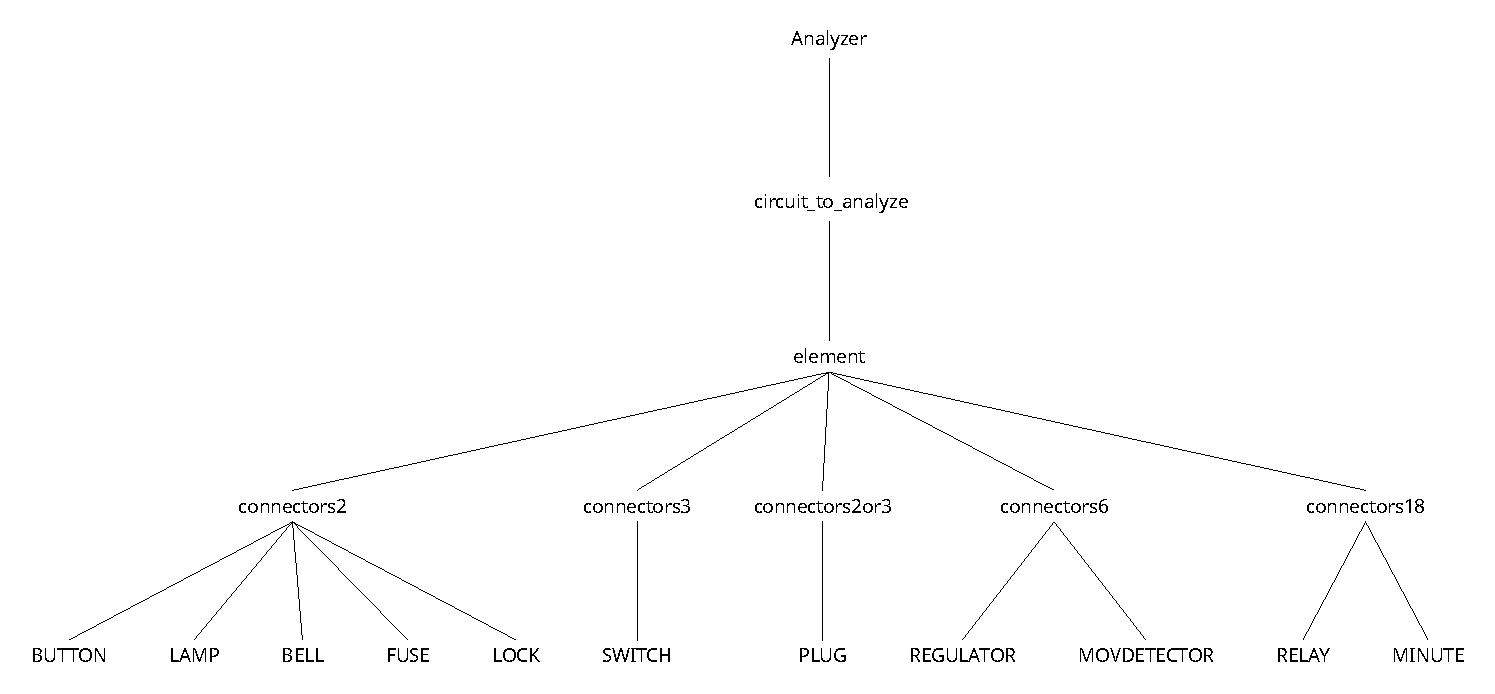
\includegraphics[scale=0.60]{Tree.pdf}
  \captionof{figure}{Versión reducida del árbol de recursión}
\end{figure}

En la figura anterior se muestra una versión muy reducida de nuestro árbol de recursión, pero sirve para hacerse una ligera idea del funcionamiento. Realmente, existen reglas intermedias que sirven para las conexiones de cada componente. Pongamos un ejemplo básico. $$\textit{lamp01(button01,button02)}$$

En este caso, tenemos una regla inicial que es \textit{analyzer}, desde aquí, se va a \textit{circuit\_to\_analyze}, y como existe un componente, se pasa a la regla \textit{element}. Obsérvese que la lámpara es un componente con dos pines y, por lo tanto, en \textit{element} se llama a la regla \textit{connectors2}. Volviendo atrás, en la regla \textit{element} se llama del mismo modo a la regla \textit{contentT1} para los token button01 y button02. Estos pulsadores llamarán de forma recursiva a las reglas en las que se contemplan los distintos componentes electrónicos, para comprobar si están conectados a R o a S, verificando de este modo, que el circuito es correcto.

Entrando un poco más en la implementación, se ha utilizado una estructura a la que se ha denomidado \texttt{connector}, que contiene un vector en el que se guardan el nombre de los elementos y los componentes a los que están conectados, junto con dos variables \texttt{R} y \texttt{S}, que indican si el elemento en cuestión, está conectado a dichas tomas. Por tanto, el vector de \texttt{connector} representa el circuito completo.

Se utiliza además esta estructura de datos para comprobar que el circuito es correcto de dos formas, la primera es que no haya componentes definidos con el mismo nombre y segundo, comprobando que cada elemento está conectado a R y a S. Todo esto, se puede resumir en el código utilizado, que se puede observar en la siguiente página:

\newpage

\newgeometry{left=2.5cm,bottom=1.5cm, top=1.5cm, right=2.5cm}

\begin{lstlisting}[basicstyle=\footnotesize]
analyzer : circuit_to_analyze;

circuit_to_analyze : | element circuit_to_analyze ;

connectors2 : BUTTON {aux.ctr.push_back(*$1);}
              | LAMP {aux.ctr.push_back(*$1);}
              | BELL {aux.ctr.push_back(*$1);}
              | FUSE {aux.ctr.push_back(*$1);}
              | LOCK {aux.ctr.push_back(*$1);};

connectors3 : SWITCH {aux.ctr.push_back(*$1); isAplug = false;};

connectors2or3 : PLUG {aux.ctr.push_back(*$1); isAplug = true;};

connectors6 : REGULATOR {aux.ctr.push_back(*$1);}
              | MOVDETECTOR {aux.ctr.push_back(*$1);};

connectors18 : RELAY {aux.ctr.push_back(*$1);}
              | MINUTE {aux.ctr.push_back(*$1);};

contentT1 : connectors2 | connectors3 | connectors2or3 | connectors6 | connectors18
              | R {aux.ctr.push_back(*$1); aux.R=*$1;}
              | S {aux.ctr.push_back(*$1); aux.S=*$1;}
              | INVALID {error=true;};

contentT2 : contentT1 | G {aux.ctr.push_back(*$1);};

morecontentT1 :  contentT1 ',' contentT1 ')' {limit+=2;}
                | contentT1 ',' contentT1  ',' morecontentT1 {limit+=2;}
                | contentT1 ')'
                { limit+=1;
                  std::string typeError = aux.ctr[0]+" has an odd number of pins";
                  error = true; yyerror(typeError.c_str());};
morecontentT2 : ')' {has3=false;}| ',' contentT2 ')' {has3=true;};

element : connectors2 '(' contentT1 ',' contentT1 ')'
          {circuit.push_back(aux); aux=connector();}
          | connectors3 '(' contentT2 ',' contentT2 ',' contentT2 ')'
          {circuit.push_back(aux); aux=connector();}

          | connectors2or3 '(' contentT2 ',' contentT2 morecontentT2
          {circuit.push_back(aux); aux=connector();
           if (isAplug&&has3) {
             if (aux.ctr[3]!="G") {
               std::string typeError = aux.ctr[0]+" is not connected to G";
               error = true; yyerror(typeError.c_str());
             }
           }
          }

          | connectors6 '(' contentT1 ',' contentT1 ',' contentT1 ','
                            contentT1 ',' contentT1 ',' contentT1 ')'
          {circuit.push_back(aux); aux=connector();}

          | connectors18 '(' morecontentT1
          {circuit.push_back(aux); aux=connector();
           if (limit>18) {
             std::string typeError = aux.ctr[0]+" has more than 18 pins";
             error = true; yyerror(typeError.c_str());
           } else {
             if (limit<4) {
               std::string typeError = aux.ctr[0]+" has less than 4 pins";
               error = true; yyerror(typeError.c_str());
             } else {limit = 0;}
           }
          }
\end{lstlisting}

\restoregeometry

\newpage


\end{document}
